\chapter{Testing and Experimental Analysis and Results}\label{ch:results}

This chapter reports the automated tests of the software, the experimental datasets, the evaluation of the deployed baseline and the experimental candidate, and a qualitative comparison with the earlier implementation on our own recordings.

\section{Unit Testing}\label{sec:ch6-tests}
The software is tested with pytest. The suite has 1,101 tests in 45 test files. In the full configuration, which includes the tests that load the real checkpoint and use the GPU, all 1,101 tests passed in 115.80 s on the development laptop (Windows 11, Python 3.10.0, pytest 9.1.1, RTX 4060 Laptop GPU), with one deprecation warning; a repeated full run also passed. A fast subset that uses a fake detector and needs no GPU is selected with \texttt{pytest -m "not slow"}. Table~\ref{tab:ch6-test-counts} gives the tests by area.

\begin{table}[!htbp]
\centering
\small
\renewcommand{\arraystretch}{1.2}
\begin{tabular}{|L{4.4cm}|L{7.4cm}|r|}
\hline
\textbf{Area} & \textbf{Examples of what is checked} & \textbf{Tests} \\
\hline
Video and GPS ingestion & GPS row rejection, clipping a trace to the video, timestamps & 241 \\
\hline
Detection, tracking, pipeline & A box moving faster than its own height stays one track; short blips rejected & 112 \\
\hline
Geospatial and map building & Complete linkage cannot grow a cluster past 8 m; snapping limit & 109 \\
\hline
Road graph and routing & Detour taken only when cheaper than the pothole penalty & 110 \\
\hline
Storage and process lock & Interrupted jobs marked failed; a second lock is refused & 37 \\
\hline
API, CLI, configuration, demo & Upload limits and error codes; demo data ignored when demo mode is off & 172 \\
\hline
ML and data tooling & Conversion edge cases, leakage guard, checkpoint selection ties, AP matches Ultralytics & 320 \\
\hline
\multicolumn{2}{|r|}{\textbf{Total}} & \textbf{1,101} \\
\hline
\end{tabular}
\caption{Automated tests by area, from the pytest collection of the full suite.}
\label{tab:ch6-test-counts}
\end{table}

Most tests target one function with small inputs built in the test. One metric test guards the average-precision correction described in Section~\ref{sec:ch5-challenges}: it checks that our AP routine agrees with the Ultralytics routine on a low-recall case. Two parts are covered only indirectly: the training entry point by configuration and dry-run tests, and the evaluation scripts by unit tests of their logic.

\section{Integration Testing}
Integration tests exercise several modules together with real components other than the detector. The API tests (79) run the application through the FastAPI test client on a temporary database with a fake detector, covering upload, the job runner, status, detections, map and coverage queries, routing, the error envelope and upload limits (a 3 MB file against a 1 MB limit must return 413 and leave nothing behind). The pipeline tests write small synthetic videos with moving objects and run the complete session processing. The map-building tests run the full derived-data rebuild, and the process-lock tests check that a second server on the same database cannot disturb the live server's jobs. Detector tests and tests marked slow load the real checkpoint.

Three things are not covered. The browser interface has no JavaScript or UI behaviour tests; only two tests check that the page is served with the right cache headers. No test measures end-to-end accuracy on labelled video from our roads, because none exists. Load behaviour is not tested.

\section{Experimental Dataset}\label{sec:ch6-data}
Table~\ref{tab:ch6-sources} lists the three public datasets. For RDD2022 we used five subsets (India, Japan, Czech Republic, United States, China MotorBike), 27,823 labelled images; China Drone was left out as not forward-facing and Norway because its very wide frames would shrink potholes to a few pixels at 640 px. The official RDD2022 test images are unlabelled, so our RDD2022 test split is an internal split of labelled images. HRP4K images were resized from $3840\times2160$ to $1280\times720$, at which the median box (square root of its area) is 20.1 px. Figure~\ref{fig:ch6-hrp-examples} shows typical HRP4K frames.

\begin{table}[!htbp]
\centering
\small
\renewcommand{\arraystretch}{1.2}
\begin{tabular}{|L{2.5cm}|L{5.4cm}|L{2.8cm}|L{2.2cm}|}
\hline
\textbf{Dataset} & \textbf{Origin} & \textbf{Licence as found} & \textbf{Role} \\
\hline
RDD2022 & Arya et al.\ \cite{arya2022rdd2022}; figshare record & CC BY 4.0 / CC BY-SA 4.0 & train, val, test \\
\hline
HRP4K v1.01 & Chen et al.\ \cite{chen2026hrp4k}; Zenodo record \cite{chen2026hrp4kzenodo} & CC BY 4.0 (metadata) & train, val, test (candidate) \\
\hline
Manhole probe & Giordani et al.\ \cite{giordani2026roaddamage}, via a Kaggle mirror & Not verified & evaluation only \\
\hline
\end{tabular}
\caption{Datasets used in the experiments.}
\label{tab:ch6-sources}
\end{table}

\begin{figure}[!htbp]
\centering
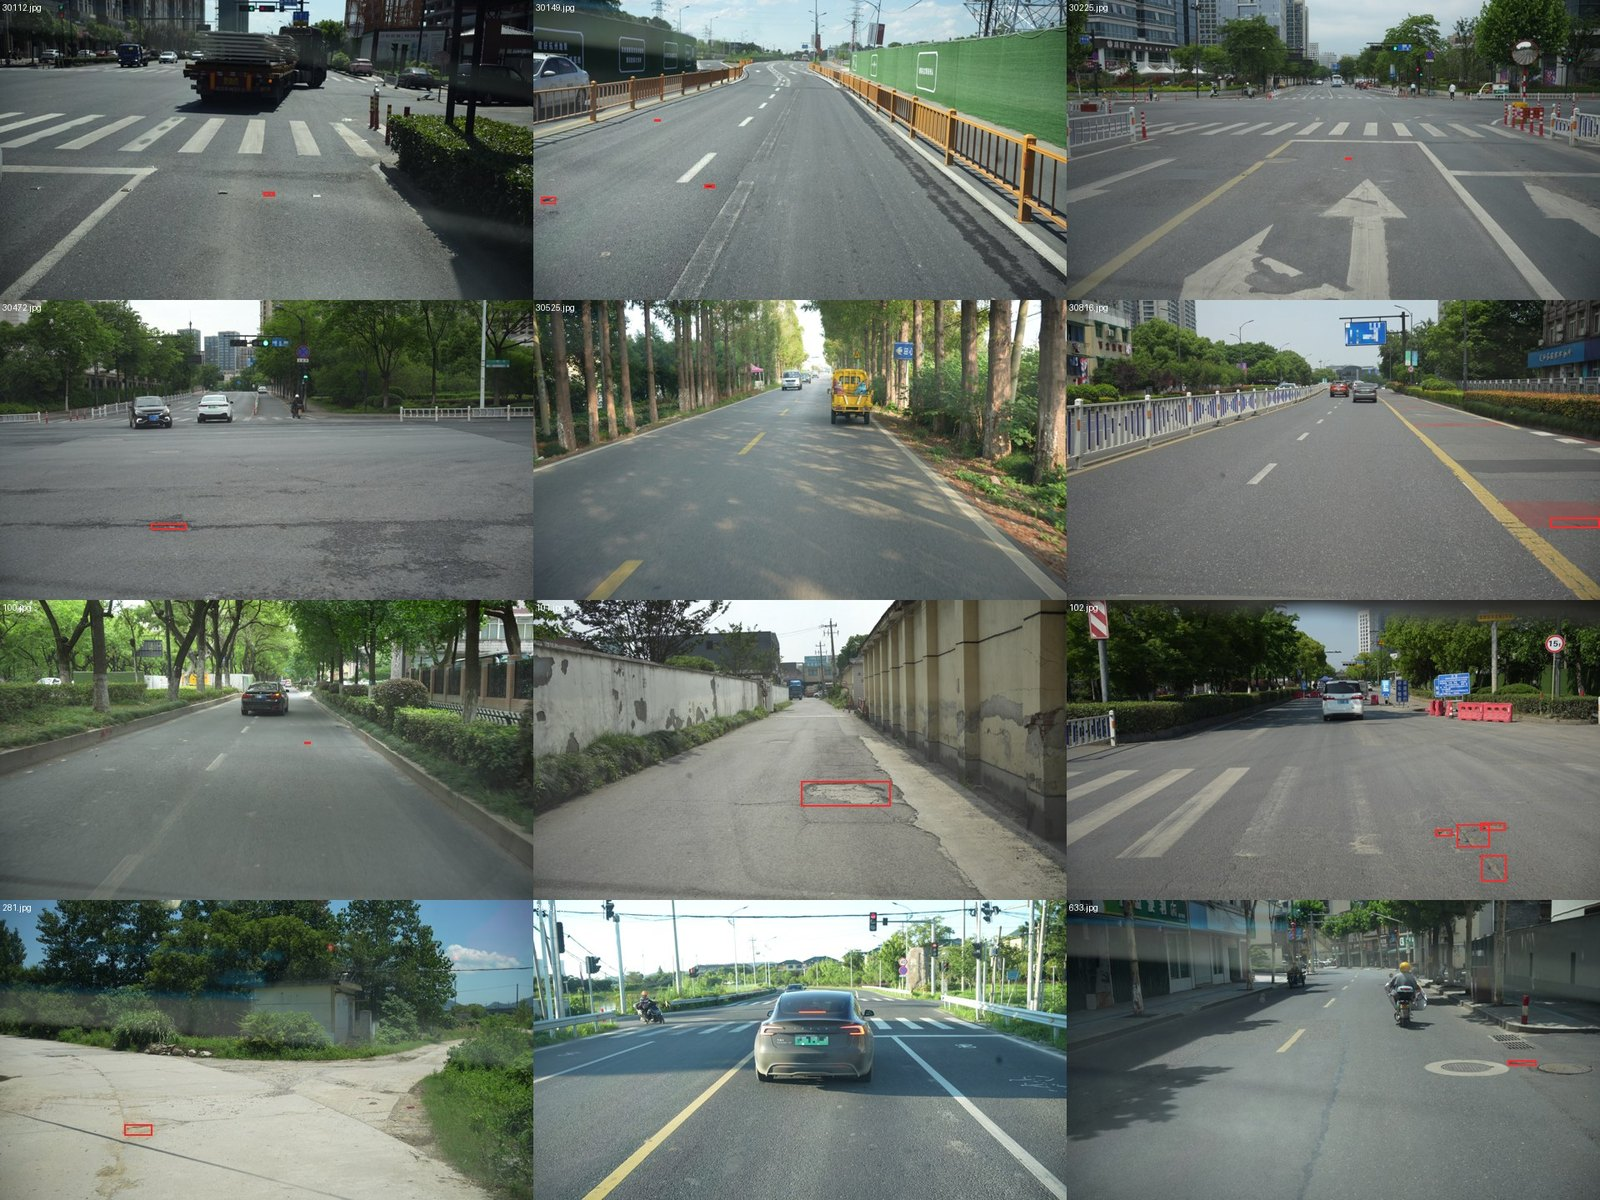
\includegraphics[width=0.55\textwidth]{ch6_hrp4k_examples.jpg}
\caption{HRP4K examples with the published boxes in red. Many potholes are only a few pixels wide at this scale. Source: HRP4K \cite{chen2026hrp4k}, CC BY 4.0 per the Zenodo metadata.}
\label{fig:ch6-hrp-examples}
\end{figure}

\subsubsection*{Review and exclusions}
The HRP4K labels were reviewed box by box in a single pass by an AI model over rendered tile sheets: of 7,217 boxes, 2,644 were judged ok, 400 rejected and 4,173 unclear. Under the exclusion-only rule, unclear boxes were kept and images with a clearly wrong box (a cover, kerb, marking, crack or patch) were excluded whole. There was no second reviewer and no agreement measure, so label noise remains: in a visual sample of 120 positive images, only about 92 of roughly 212 boxes clearly lay on a pothole. The manhole probe was reviewed more strictly and keeps 42 images with potholes plus 161 pothole-free images that each contain an intact manhole; its false-alarm rate therefore measures behaviour on manholes, not general behaviour.

\subsubsection*{Splits and leakage}
After grouping (Section~\ref{sec:ch4-dataset}), no group spans two splits and no validation or test image has a training image within 8 bits. The HRP4K leakage guard removed 51 validation and 76 test images. Some overlap remains: about 64\% of RDD2022 validation and test images have a training image at 9 to 12 bits, mostly similar road layouts rather than the same scene, so RDD2022 scores are probably optimistic for unseen roads. Training negatives in RDD2022 were capped at two per positive image; validation and test keep their natural mix (about 11\% positive). Table~\ref{tab:ch6-composition} gives the final composition.

\begin{table}[!htbp]
\centering
\small
\renewcommand{\arraystretch}{1.2}
\begin{tabular}{|L{2.8cm}|L{2.6cm}|r|r|r|r|}
\hline
\textbf{Source} & \textbf{Split} & \textbf{Images} & \textbf{Boxes} & \textbf{Positive} & \textbf{Empty} \\
\hline
RDD2022 & train & 8,220 & 5,017 & 2,740 & 5,480 \\
\hline
RDD2022 & validation & 2,784 & 477 & 299 & 2,485 \\
\hline
RDD2022 & test & 2,784 & 503 & 315 & 2,469 \\
\hline
HRP4K & train & 3,973 & 4,709 & 2,573 & 1,400 \\
\hline
HRP4K & validation & 825 & 922 & 535 & 290 \\
\hline
HRP4K & test & 811 & 836 & 538 & 273 \\
\hline
Manhole probe & evaluation only & 203 & 59 & 42 & 161 \\
\hline
\end{tabular}
\caption{Final composition of the experimental datasets. The probe also has 196 intact manhole boxes, which are not pothole targets.}
\label{tab:ch6-composition}
\end{table}

\section{Performance Analysis}

\subsection{Evaluation protocol}\label{sec:ch6-protocol}
A prediction matches a ground-truth box if their IoU is at least 0.5, greedily by descending confidence. At a confidence threshold $t$, precision $P=TP/(TP+FP)$, recall $R=TP/N_{gt}$ and
\begin{equation}
F_1=\frac{2PR}{P+R},
\label{eq:ch6-f1}
\end{equation}
where $N_{gt}$ is the number of ground-truth boxes. We also report false positives per image and mAP\textsubscript{50} and mAP\textsubscript{50--95} with the 101-point interpolation of Ultralytics \cite{padilla2020survey}. On the probe, the \emph{manhole hit share} is the fraction of the 196 manhole boxes overlapped (IoU $\ge 0.3$) by a pothole prediction.

The threshold of each model is the one that maximises $F_1$ on the pooled RDD2022 and HRP4K validation set, and it is applied unchanged to the test sets \cite{cawley2010overfitting}: 0.2705 for the baseline at 640 px and 0.2450 for the candidate at 1280 px. In the deployed application the confidence threshold is a provisional 0.25. The intervals come from a group bootstrap \cite{efron1993bootstrap}, in which whole near-duplicate groups are resampled 1,000 times and the 2.5th and 97.5th percentiles give the 95\% interval. Because both models are scored on the same resamples, their difference can be computed pair by pair \cite{koehn2004significance}, and an asterisk marks any interval that does not include zero. We did not correct for multiple comparisons. The test splits were also evaluated more than once during development, and no log of those evaluations was kept.

\subsection{Results of the baseline model}\label{sec:ch6-results}
Early stopping ended the baseline's training after 76 epochs, and we kept the checkpoint from epoch 56. Figure~\ref{fig:ch6-curves-baseline} shows the training-time curves on the RDD2022 validation split: the metrics flatten after about epoch 50 while the validation losses rise, a sign of overfitting.

\begin{figure}[!htbp]
\centering
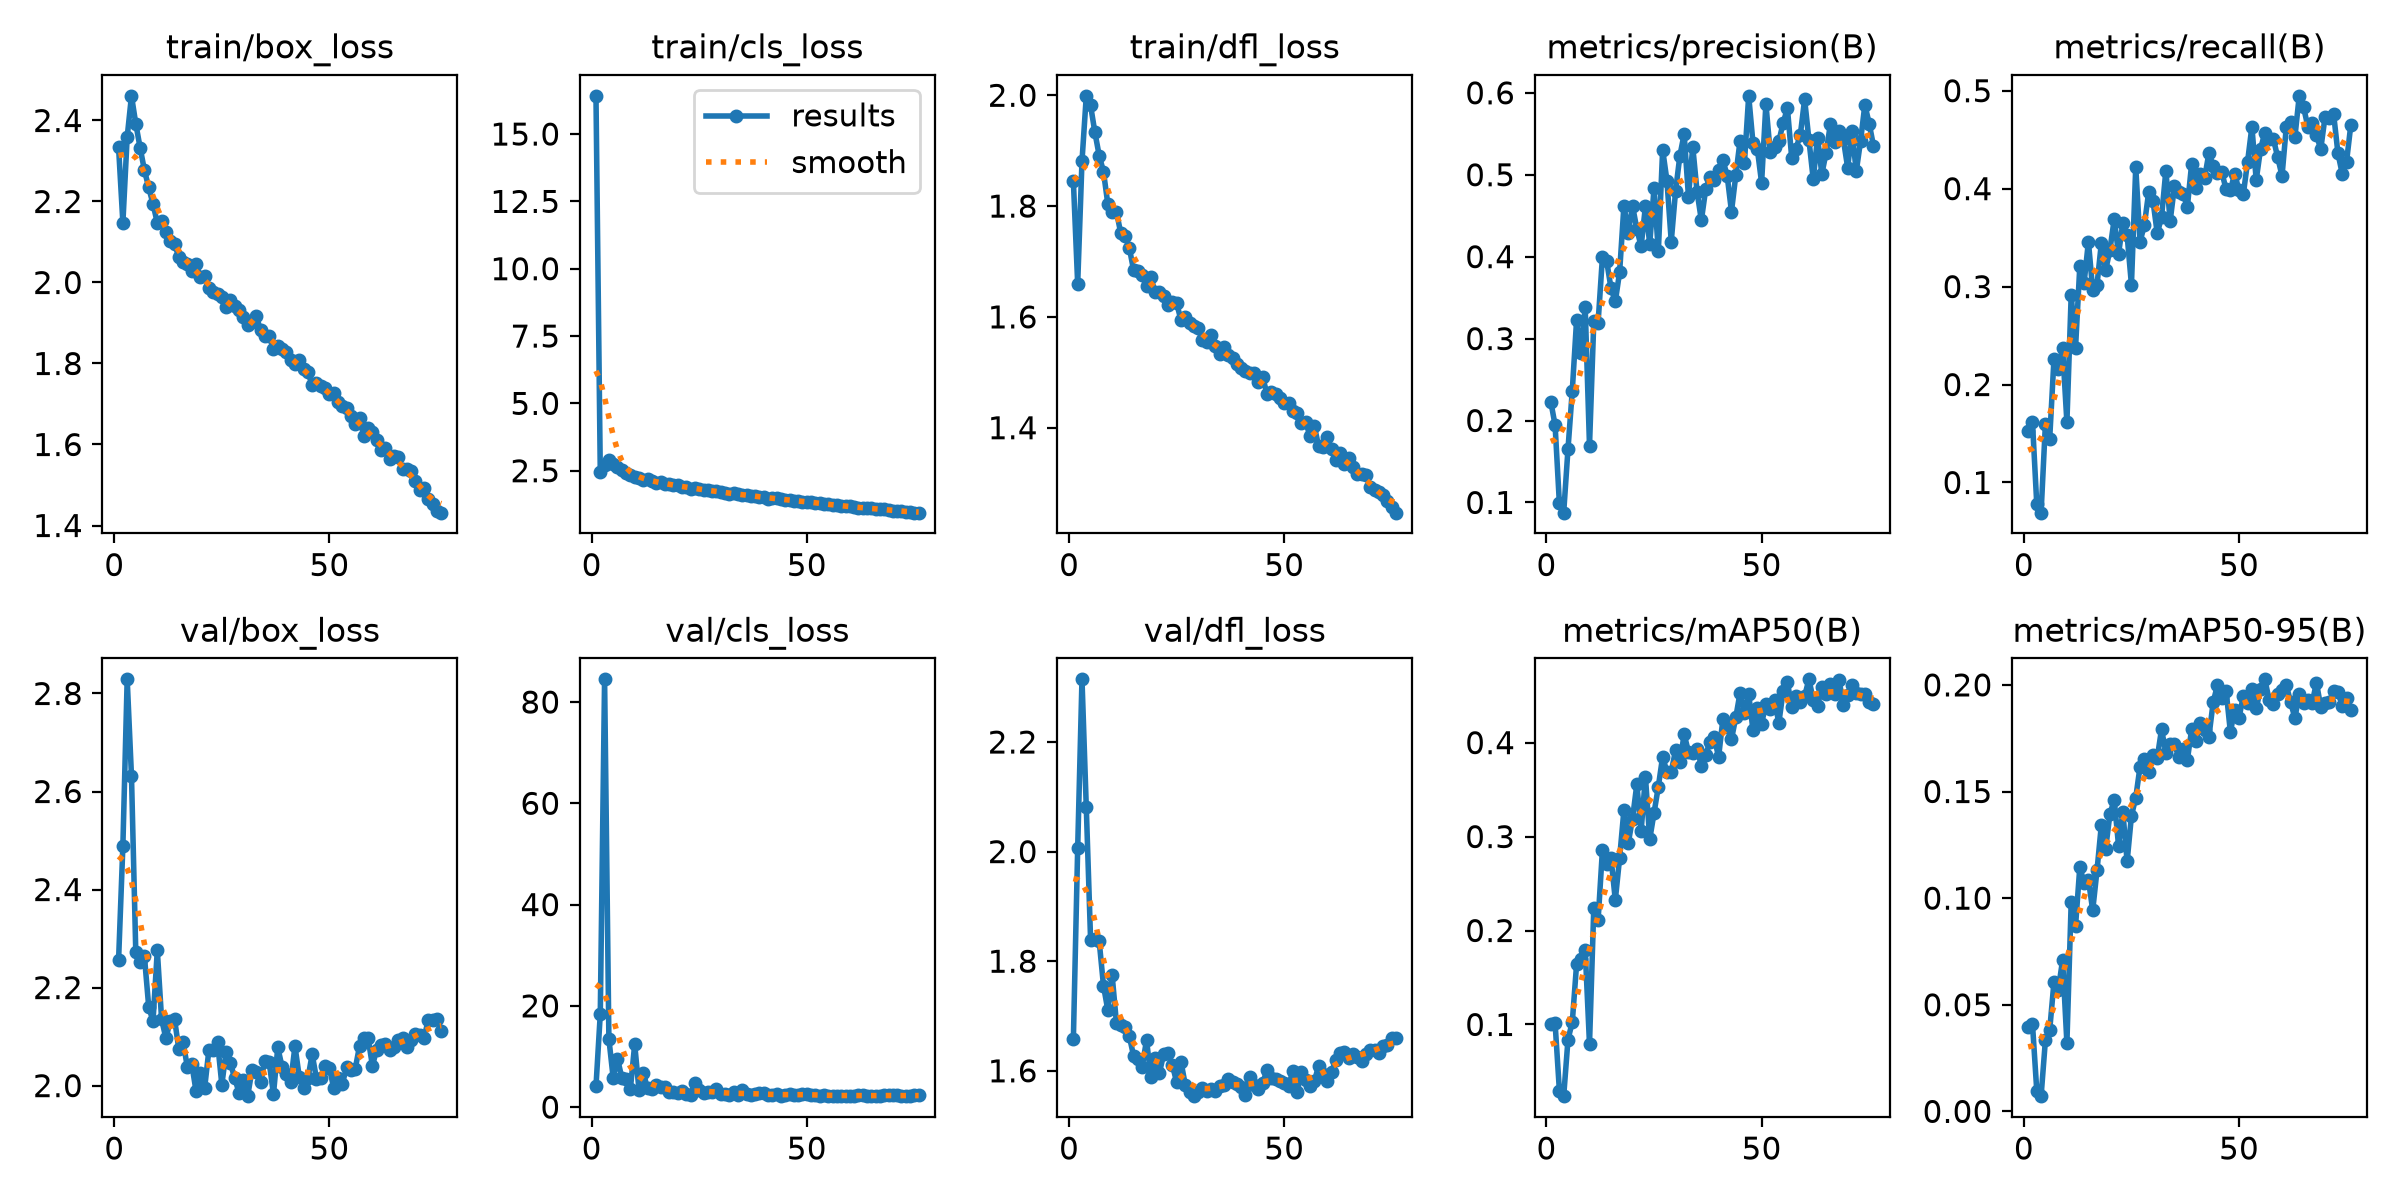
\includegraphics[width=0.72\textwidth]{ch6_train_curves_baseline.png}
\caption{Training losses and training-time validation curves of the baseline (YOLOv8s, RDD2022, 640 px, 76 epochs), as written by the training framework.}
\label{fig:ch6-curves-baseline}
\end{figure}

On the held-out RDD2022 test split (2,784 images, 503 boxes) the baseline reaches mAP\textsubscript{50} 0.497 [0.443, 0.555], mAP\textsubscript{50--95} 0.207 [0.180, 0.239], precision 0.515, recall 0.529, F\textsubscript{1} 0.522 [0.478, 0.562] and 0.090 false positives per image. On HRP4K test it reaches only mAP\textsubscript{50} 0.018, because it never saw HRP4K and the median pothole shrinks to about 10 px at 640 px input. On the manhole probe it reaches mAP\textsubscript{50} 0.368 [0.215, 0.528].

\subsection{Candidate experiment}
The candidate was fine-tuned from the baseline on RDD2022 and HRP4K at 1280 px (Table~\ref{tab:ch5-train}). Its checkpoint was chosen by a rule declared before any test evaluation: the highest mean of RDD2022 and HRP4K validation mAP\textsubscript{50}. The winner, \texttt{epoch25.pt}, led the runner-up by only about 0.0014, so the choice was effectively a tie broken by the rule. Table~\ref{tab:ch6-main} compares the two models at their own thresholds; Figure~\ref{fig:ch6-paired} plots the paired differences.

\begin{table}[!htbp]
\centering
\footnotesize
\renewcommand{\arraystretch}{1.2}
\begin{tabular}{|L{1.5cm}|L{2.4cm}|L{1.9cm}|L{1.9cm}|L{4.6cm}|}
\hline
\textbf{Set} & \textbf{Metric} & \textbf{Baseline, 640 px} & \textbf{Candidate, 1280 px} & \textbf{Difference [95\% CI]} \\
\hline
RDD2022 & mAP\textsubscript{50} & 0.497 & 0.453 & $-$0.0445 [$-$0.0864, $-$0.0059]$^{*}$ \\
\cline{2-5}
test & Precision & 0.515 & 0.454 & $-$0.0608 [$-$0.1055, $-$0.0161]$^{*}$ \\
\cline{2-5}
 & Recall & 0.529 & 0.487 & $-$0.0417 [$-$0.0823, 0.0000] \\
\cline{2-5}
 & FP per image & 0.090 & 0.106 & 0.0158 [0.0004, 0.0314]$^{*}$ \\
\hline
HRP4K & mAP\textsubscript{50} & 0.018 & 0.454 & 0.4354 [0.3915, 0.4792]$^{*}$ \\
\cline{2-5}
test & Recall & 0.019 & 0.416 & 0.3971 [0.3509, 0.4455]$^{*}$ \\
\cline{2-5}
 & FP per image & 0.075 & 0.253 & 0.1776 [0.1304, 0.2278]$^{*}$ \\
\hline
Manhole & mAP\textsubscript{50} & 0.368 & 0.427 & 0.0581 [$-$0.0267, 0.1945] \\
\cline{2-5}
probe & FP per image & 0.222 & 0.291 & 0.0690 [$-$0.0140, 0.1429] \\
\cline{2-5}
 & Manhole hit share & 0.133 & 0.148 & 0.0153 [$-$0.0657, 0.0762] \\
\hline
\end{tabular}
\caption{Results of the baseline and the candidate on the held-out test splits and the manhole probe, each model at the threshold chosen for it on pooled validation data. Each difference is the candidate's value minus the baseline's over paired group-bootstrap resamples, and $^{*}$ marks intervals that do not contain zero. Only the candidate was trained on HRP4K data.}
\label{tab:ch6-main}
\end{table}

\begin{figure}[!htbp]
\centering
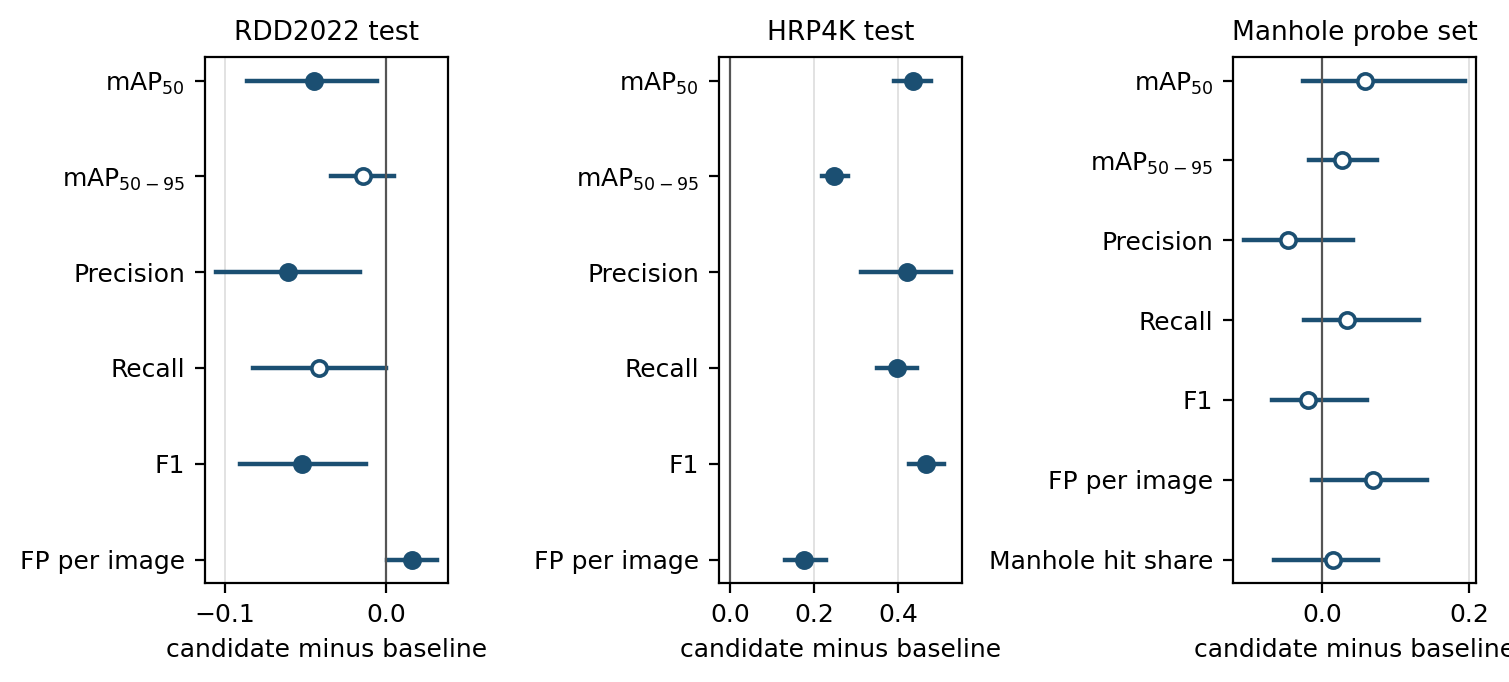
\includegraphics[width=0.95\textwidth]{ch6_paired_differences.png}
\caption{Difference between the candidate and the baseline for each metric, with its 95\% group-bootstrap interval. Filled markers show intervals that do not contain zero, and the panels use different horizontal scales.}
\label{fig:ch6-paired}
\end{figure}

\subsubsection*{Same-resolution checks}
The main comparison mixes data, training and input size. With both models at 640 px, the candidate's RDD2022 test mAP\textsubscript{50} is 0.491 (difference $-$0.0060 [$-$0.0449, 0.0331], not distinguishable), but its precision is lower ($-$0.0898$^{*}$) and it produces more false positives on RDD2022 (+0.0402$^{*}$) and on the probe (0.320 against 0.222 per image$^{*}$); its HRP4K mAP\textsubscript{50} is 0.313 against 0.018. With both at 1280 px, the candidate looks better everywhere, including a lower manhole hit share (0.148 against 0.316), but the baseline is then running at a size it was not trained for, so this is not evidence about the deployed system.

\subsubsection*{Latency}
On the RTX 4060 Laptop GPU (batch 1, forward pass and NMS), the baseline and candidate take 8.16 and 8.19 ms at 640 px in FP32, 17.44 and 16.65 ms at 1280 px in FP32, and 11.02 and 10.62 ms at 1280 px in FP16. Both are YOLOv8s, so cost depends on input size, not on the weights.

\subsection{Interpretation}
The candidate's large gain on HRP4K (mAP\textsubscript{50} 0.018 to 0.454) reflects that it was trained on HRP4K while the baseline never saw it, together with the larger input; it is not a general improvement. At 640 px the candidate still reaches 0.313 on HRP4K, so the gain does not depend on resolution alone, but a single run cannot divide the effect between data and resolution. On RDD2022, which both models were trained on, the candidate is somewhat worse: lower mAP\textsubscript{50}, precision and F\textsubscript{1}, and more false positives per image. We did not demonstrate that the candidate reduces false positives or confusion with manholes compared with the deployed baseline: on the probe the differences have intervals that include zero, and the probe is small (59 pothole boxes, 63 groups). The only comparison favouring the candidate on false positives uses the baseline outside its training resolution. The candidate also differs in data, input size, optimiser and schedule, so one run cannot attribute effects to causes.

\subsection{Validation-only investigations}
Three investigations used validation data only and changed no decision. The candidate's F\textsubscript{1} curve is flat near its peak, staying within 0.01 of the maximum for thresholds from 0.18 to 0.33, and cross-fitting showed that selecting the threshold in-sample is optimistic by only about 0.003 to 0.006 in F\textsubscript{1}. Weighted boxes fusion \cite{solovyev2021wbf} of the baseline at 640 px and the candidate at 960 px gave the same F\textsubscript{1} as the baseline alone on RDD2022 validation (difference 0.001 [$-$0.031, 0.029]) and fell below the candidate on HRP4K validation while costing an extra forward pass, so no ensemble is deployed. Finally, of the candidate's 260 false positives on HRP4K validation, 240 poorly localised or background boxes were categorised in one visual AI pass (Table~\ref{tab:ch6-fp-categories}). Manhole covers account for only 6 (2.5\%), so this analysis does not support manhole confusion as the main error source on HRP4K; 8 boxes appear to lie on unlabelled potholes.

\begin{table}[!htbp]
\centering
\small
\renewcommand{\arraystretch}{1.15}
\begin{tabular}{|l|r|l|r|}
\hline
\textbf{Category} & \textbf{Boxes} & \textbf{Category} & \textbf{Boxes} \\
\hline
Unclear & 101 & Shadow, stain or wet area & 12 \\
\hline
Crack or surface wear & 36 & Plausible unlabelled pothole & 8 \\
\hline
Patch or repair & 32 & Manhole or utility cover & 6 \\
\hline
Road edge or off-road & 27 & Debris or object & 4 \\
\hline
Road marking & 13 & Drain or grate & 1 \\
\hline
\end{tabular}
\caption{Categories of 240 candidate false positives on HRP4K validation images (single AI visual pass; not ground truth).}
\label{tab:ch6-fp-categories}
\end{table}

\subsection{Qualitative comparison on own recordings}
Our 13 recordings from Bengaluru ($1280\times720$, about 30 frames per second, 9,711 frames in total) have no ground truth. Everything in this subsection describes model behaviour and is not a measurement of accuracy, precision, recall or false-positive rate; a higher detection count does not indicate a better model. We ran three models on every frame: the earlier implementation's YOLOv8s-seg model (boxes only, at its own confidence of 0.35, without its stride-5 sampling and ByteTrack tracking), the baseline and the candidate at their validation-selected thresholds. Table~\ref{tab:ch6-totals} gives the totals and Table~\ref{tab:ch6-agreement} the frame-level detection presence.

\begin{table}[!htbp]
\centering
\small
\renewcommand{\arraystretch}{1.15}
\begin{tabular}{|L{4.0cm}|r|r|r|}
\hline
\textbf{Model} & \textbf{Detections} & \textbf{Frames with a detection} & \textbf{Median confidence} \\
\hline
Earlier implementation & 9,665 & 77.29\% & 0.722 \\
\hline
Baseline & 1,913 & 15.91\% & 0.506 \\
\hline
Candidate & 3,049 & 21.73\% & 0.418 \\
\hline
\end{tabular}
\caption{Detections over the 13 recordings (9,711 frames). Behaviour only; no ground truth.}
\label{tab:ch6-totals}
\end{table}

\begin{table}[!htbp]
\centering
\small
\renewcommand{\arraystretch}{1.15}
\begin{tabular}{|L{5.4cm}|r|L{4.6cm}|r|}
\hline
\textbf{Models that fire in the frame} & \textbf{Frames} & \textbf{Models that fire} & \textbf{Frames} \\
\hline
None & 1,537 & Earlier and baseline only & 416 \\
\hline
Earlier implementation only & 5,479 & Earlier and candidate only & 883 \\
\hline
Baseline only & 169 & Baseline and candidate only & 232 \\
\hline
Candidate only & 267 & All three & 728 \\
\hline
\end{tabular}
\caption{Frame-level detection presence of the three models (9,711 frames). These are presence statistics, not accuracy measurements.}
\label{tab:ch6-agreement}
\end{table}

The earlier model fires in most frames, and 3,107 of its 9,665 boxes cover at least 80\% of the frame, which is consistent with the over-segmentation that the Phase 1 report itself recorded on forward-facing footage; neither new model produced such a box. The baseline and the candidate agree on whether a frame contains a detection in 82.13\% of frames. Review strips (Figures~\ref{fig:ch6-strip-pothole} and~\ref{fig:ch6-strip-cover}) were hand-picked to include cases unfavourable to each model and are not representative. In sampled frames both new models also fire on flush manhole covers, patches, stains and paint, so they are not free of look-alike errors, and a visual review of the sampled frames found no clear overall winner between the baseline and the candidate.

\begin{figure}[!htbp]
\centering
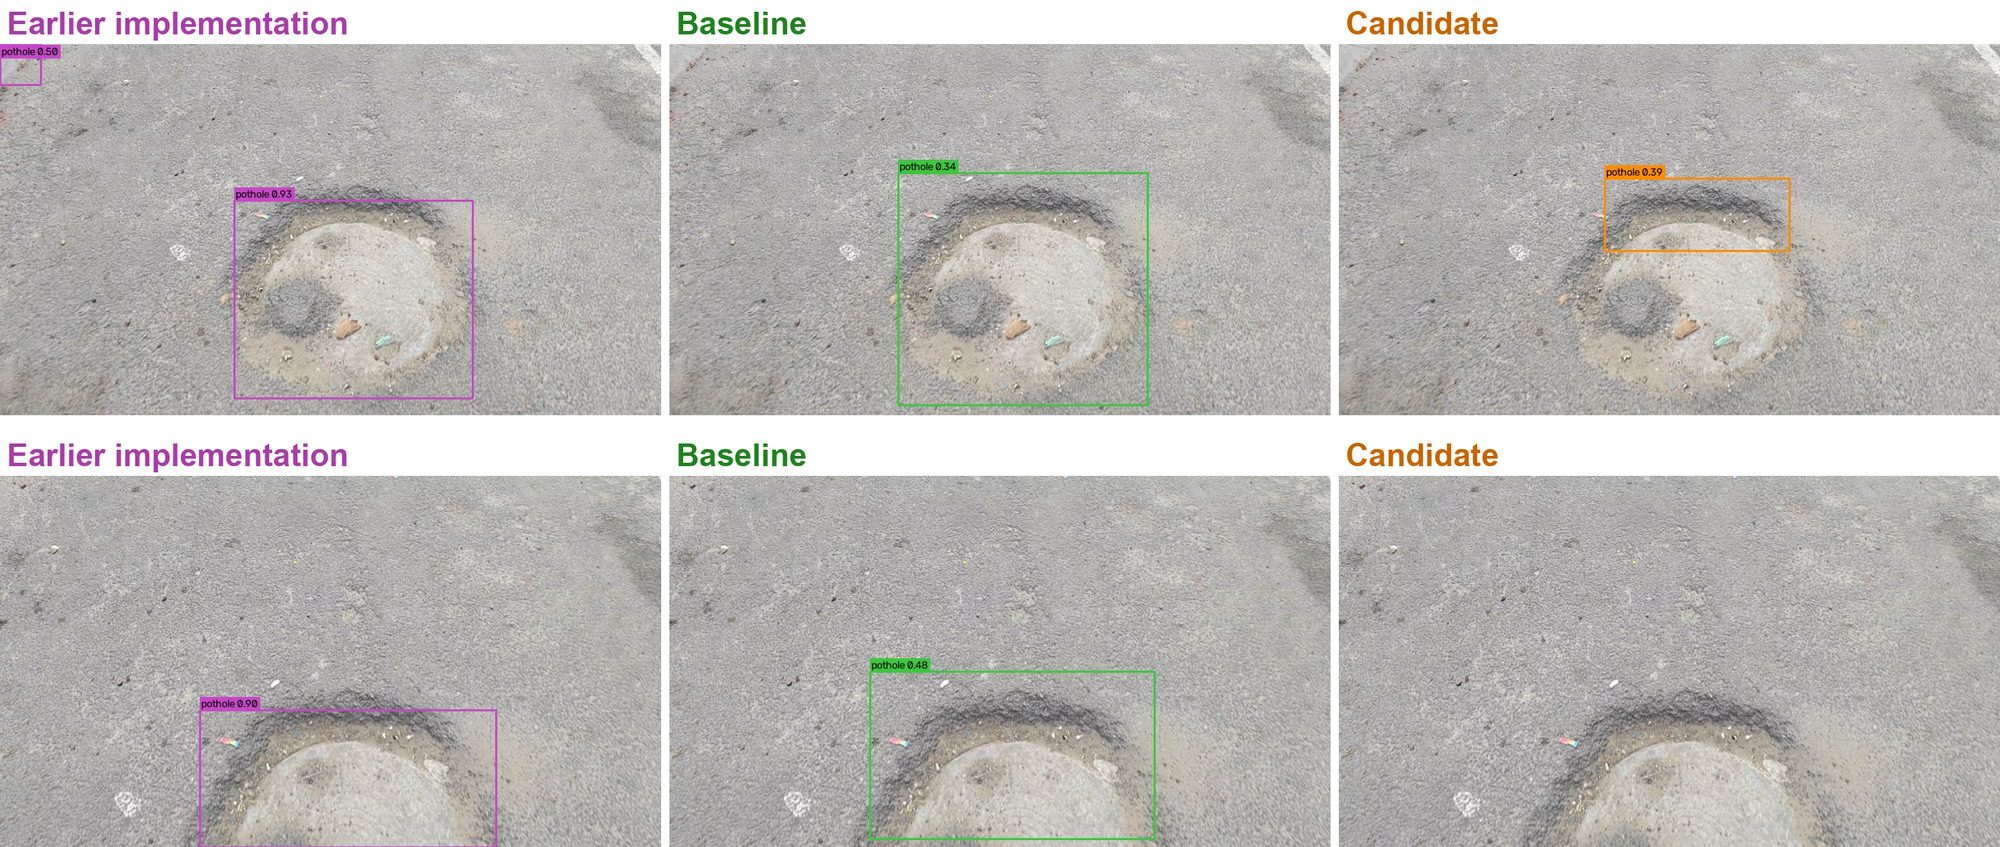
\includegraphics[width=0.82\textwidth]{ch6_strips_round_pothole.jpg}
\caption{Review strip (hand-picked, not representative): a round sunken area of road in two frames of one recording, processed by the earlier implementation, the baseline and the candidate. This is a qualitative view only, since these frames have no ground-truth labels.}
\label{fig:ch6-strip-pothole}
\end{figure}

\begin{figure}[!htbp]
\centering
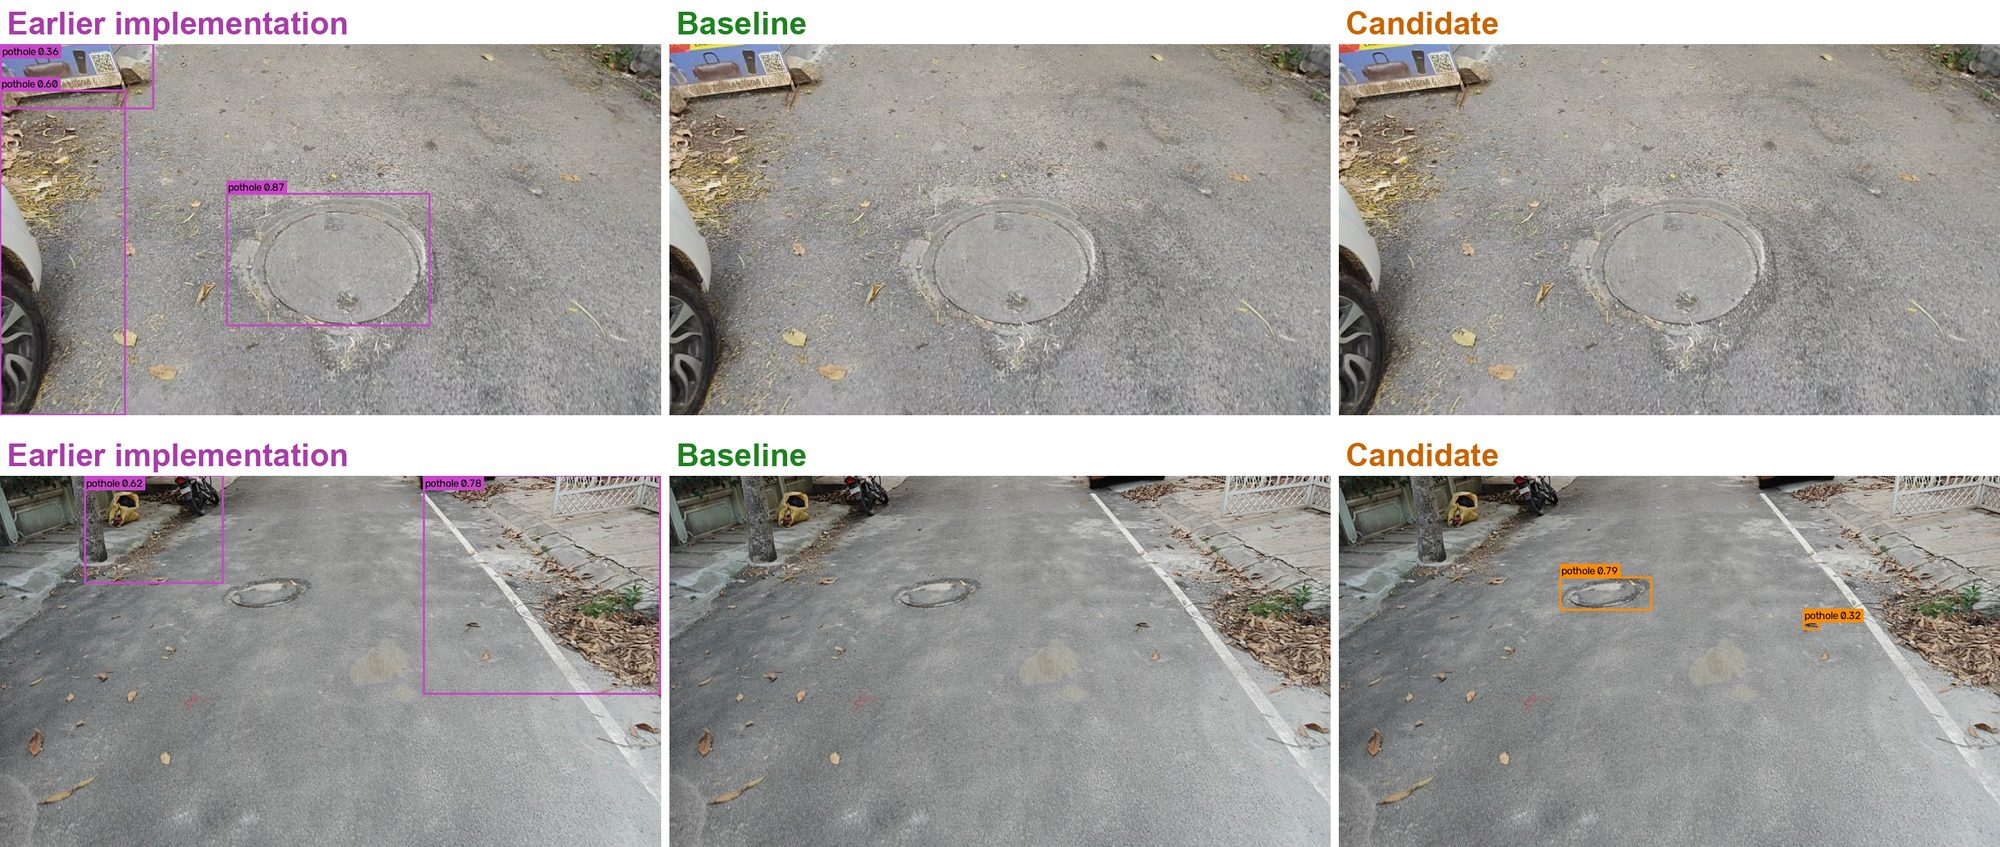
\includegraphics[width=0.82\textwidth]{ch6_strips_manhole_cover.jpg}
\caption{Hand-picked frames, not representative, showing manhole covers set flush with the road in two of our recordings. In the lower frame the candidate draws a box on the cover. These frames have no ground-truth labels, so the comparison is qualitative.}
\label{fig:ch6-strip-cover}
\end{figure}

\subsection{Limitations}
\begin{itemize}[itemsep=0pt]
\item The candidate is one training run with one seed; HRP4K was in-domain for it and was also used to select its epoch and threshold.
\item Label review was a single automated pass that only excluded images; 58\% of HRP4K boxes were judged unclear and kept, and label noise remains.
\item The manhole probe is small (203 images, 63 groups), and all its pothole-free frames contain a manhole by construction.
\item RDD2022 retains scene-level similarity between splits, so its scores are probably optimistic; several country subsets have very few positive test images.
\item No correction for multiple comparisons was applied across the many intervals, and the test splits were evaluated more than once without a log of each run.
\item Our recordings have no ground truth, so no accuracy is known on the roads the system targets.
\item The thresholds of the deployed pipeline, including the 0.25 confidence, the tracking parameters and the 8 m merge radius, are provisional and were never tuned. When we went through 50 confirmed tracks by eye, we judged 8 to be plausible potholes, 11 other road damage, 18 clear false positives and 13 unclear, a subjective count.
\item Route comparison has only been shown on a synthetic session. The system also serves a single user, has no authentication and processes one job at a time.
\end{itemize}

\subsection{Outcome}
We are keeping the baseline as the deployed model. The candidate stays as an experiment, because its only clear gain is on HRP4K, the data it was trained on. On RDD2022 it is somewhat worse, and it did not show fewer false positives or less confusion with manholes. Before the baseline could be replaced, we would need labelled frames from our own roads.
